% ---------------------------------------------------------------
% Section: Detection Benchmarks — trackpy vs LodeSTAR
% ---------------------------------------------------------------

\section[Detection Benchmarks]{Detection Benchmarks: trackpy vs LodeSTAR}

\begin{frame}{Detection Engine Benchmark}
\begin{columns}
\begin{column}{0.58\textwidth}
\begin{figure}
    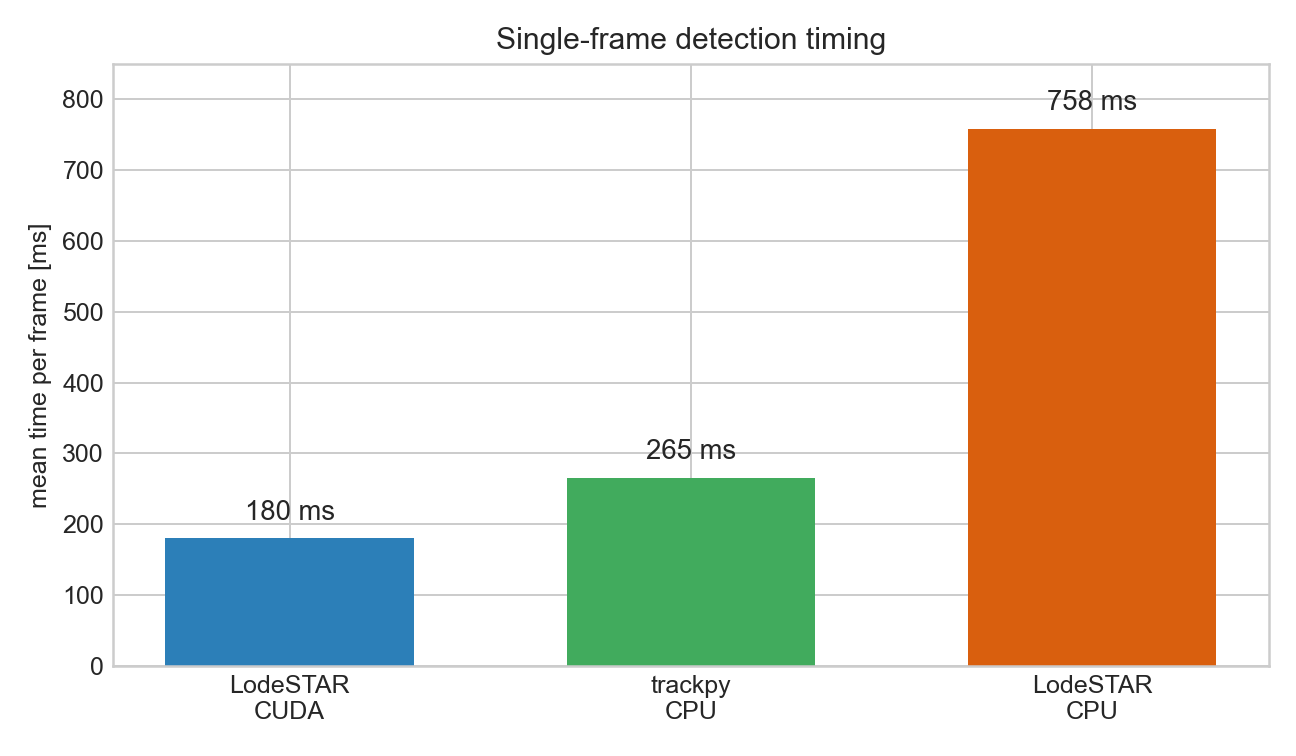
\includegraphics[width=\textwidth]{imglib/progress_update/detection_timing_bar.png}
\end{figure}
\end{column}
\begin{column}{0.42\textwidth}
\begin{myalert}[Takeaway]
\small LodeSTAR is the faster detector only when CUDA is available; trackpy remains the CPU baseline.
\end{myalert}
\smallskip
\begin{mynote}
\footnotesize One 1024$\times$1024 JP frame, 30 timed reps after warmup.
\end{mynote}
\end{column}
\end{columns}
\end{frame}

\begin{frame}{Do the Engines Agree?}
\begin{columns}
\begin{column}{0.66\textwidth}
\begin{figure}
    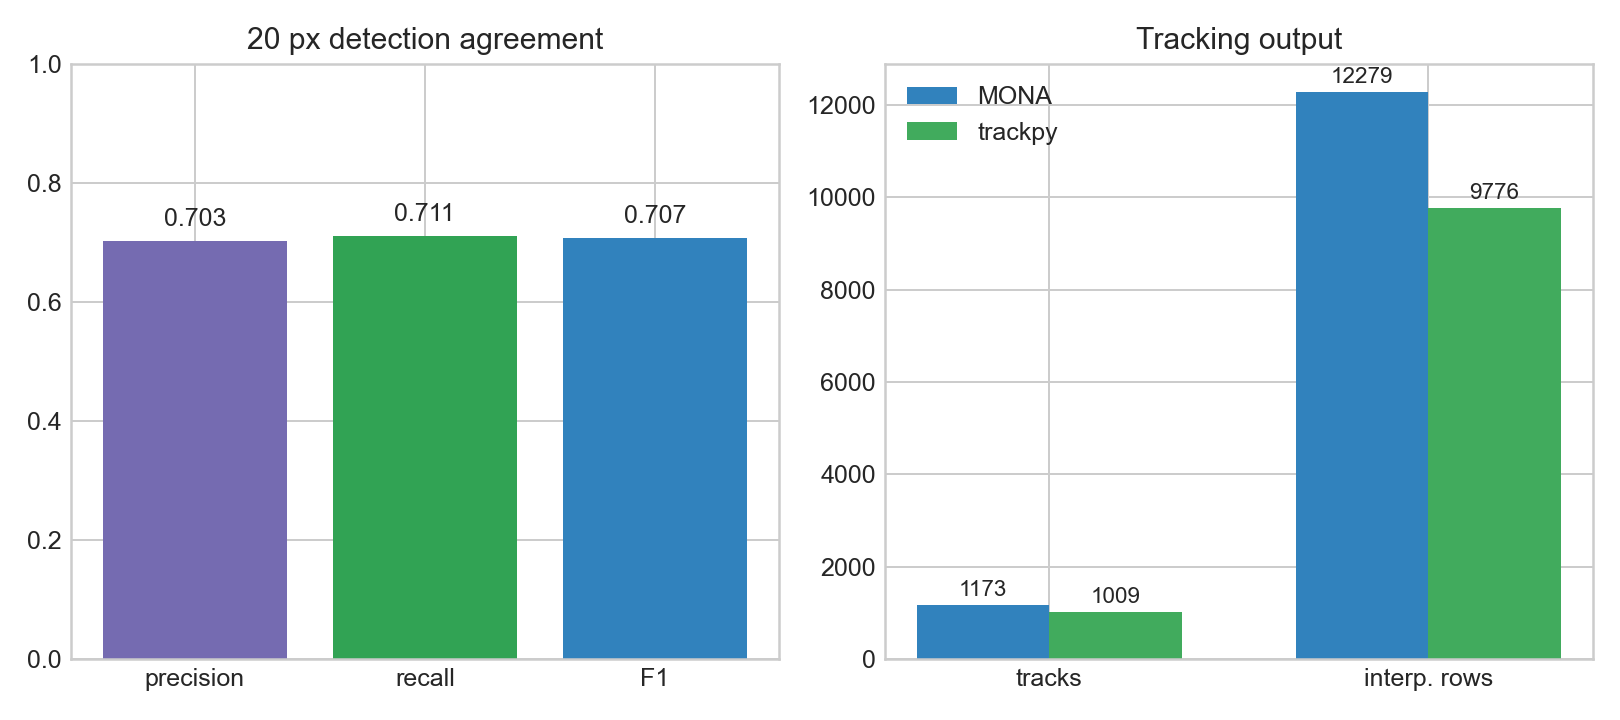
\includegraphics[width=\textwidth]{imglib/progress_update/detection_agreement_tracking.png}
\end{figure}
\end{column}
\begin{column}{0.34\textwidth}
\begin{myalert}[Not interchangeable]
\small $\sim$71\% agreement within 20 px; mean matched distance is 4.09 px.
\end{myalert}
\smallskip
\begin{mynote}
\footnotesize Trackpy is a reference detector here, not ground truth.
\end{mynote}
\end{column}
\end{columns}
\end{frame}

\begin{frame}{Run \texttt{04}: Benchmark Summary}
\begin{columns}
\begin{column}{0.62\textwidth}
\begin{figure}
    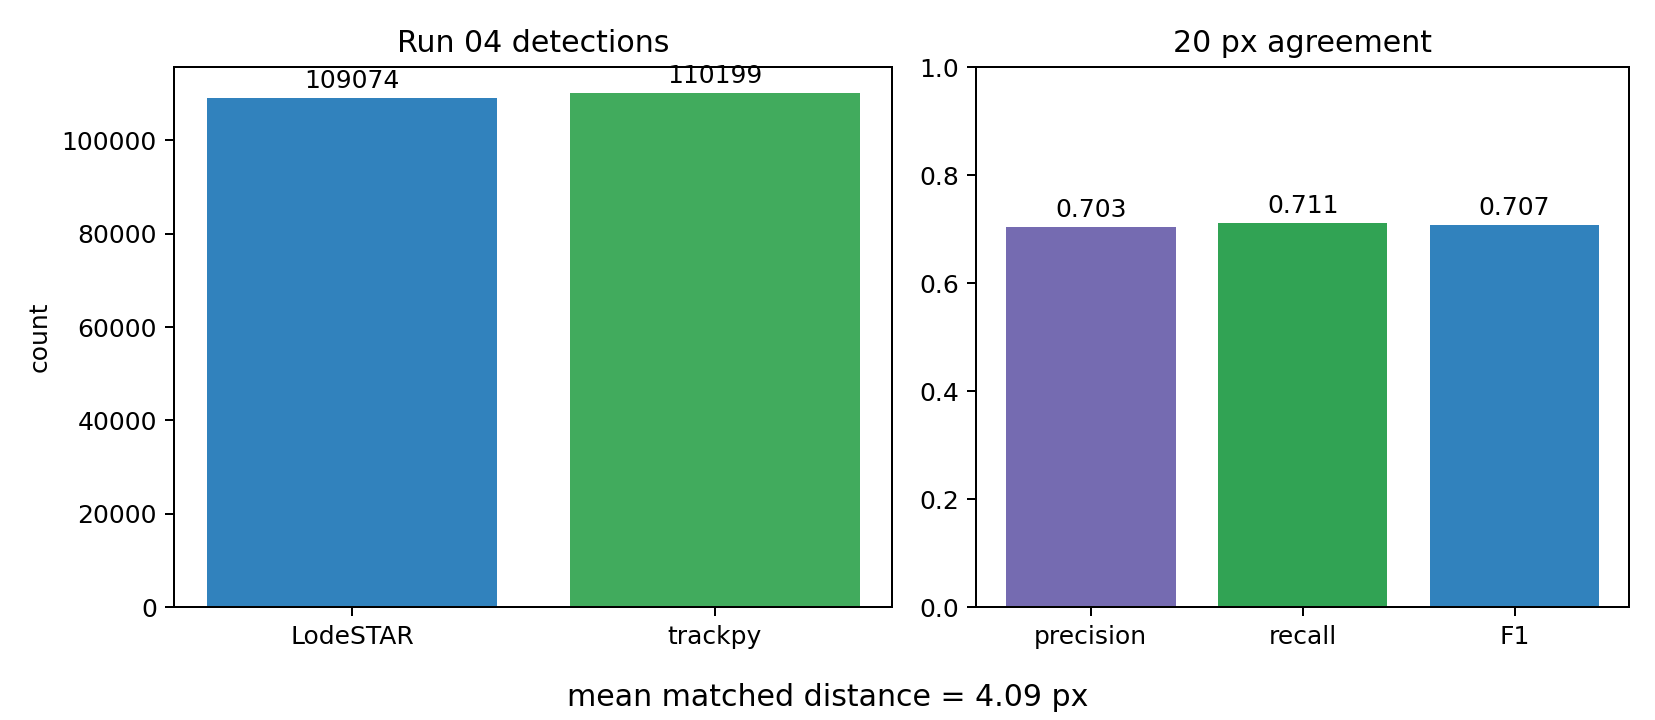
\includegraphics[width=\textwidth]{imglib/progress_update/run04_trackpy_lodestar_benchmark.png}
\end{figure}
\end{column}
\begin{column}{0.38\textwidth}
\begin{myalert}[Benchmark dir]
\small Agreement is close enough for comparison, but not close enough to treat trackpy and LodeSTAR tracks as interchangeable.
\end{myalert}
\end{column}
\end{columns}
\end{frame}

\begin{frame}{Run \texttt{04}: Detection-to-Tracking Visual Check}
\begin{columns}
\begin{column}{0.5\textwidth}
\begin{figure}
    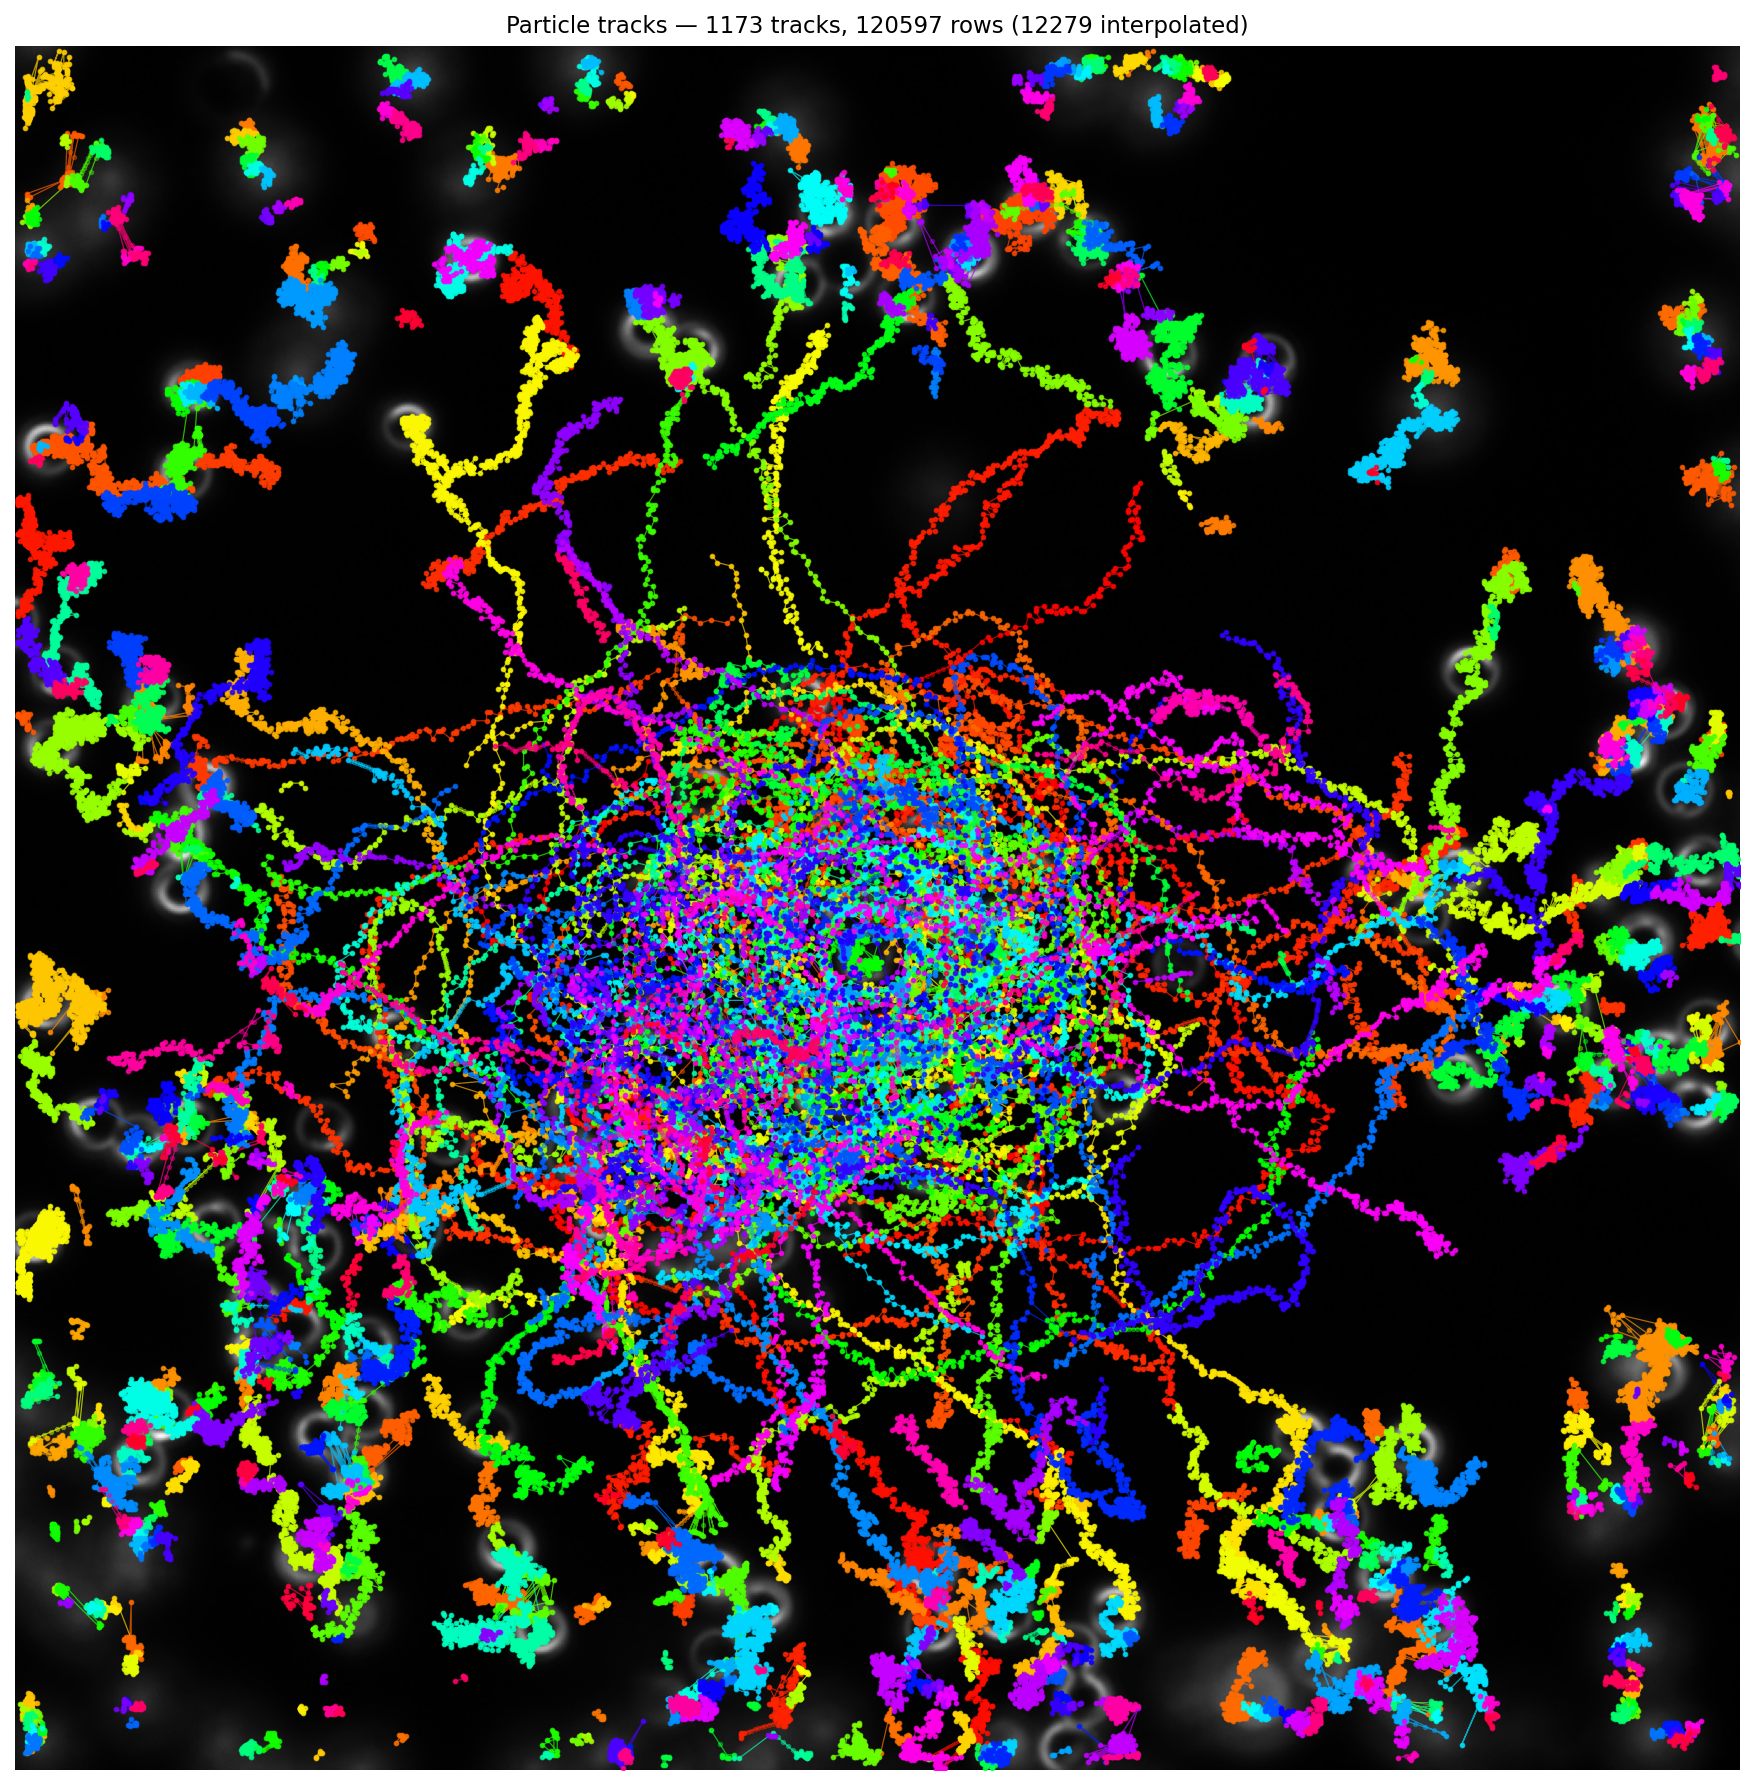
\includegraphics[width=\textwidth, height=0.72\textheight, keepaspectratio]{imglib/progress_update/run04_lodestar_tracks_overview.png}
\end{figure}
\end{column}
\begin{column}{0.5\textwidth}
\begin{figure}
    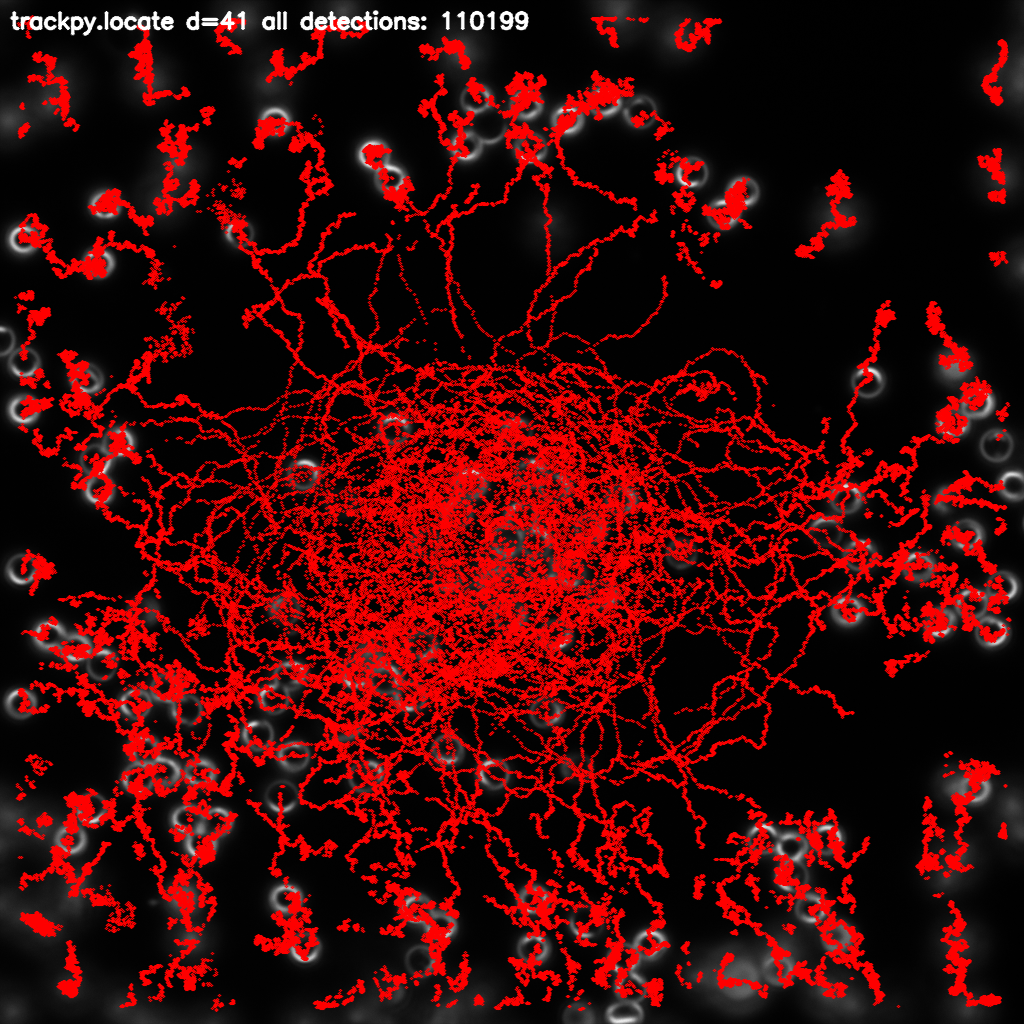
\includegraphics[width=\textwidth, height=0.72\textheight, keepaspectratio]{imglib/progress_update/run04_trackpy_locate_overview.png}
\end{figure}
\end{column}
\end{columns}
\end{frame}
